\section{mo\-LSCheck\-Point$<$ M $>$ Class Template Reference}
\label{classmo_l_s_check_point}\index{moLSCheckPoint@{moLSCheckPoint}}
Class which allows a checkpointing system.  


{\tt \#include $<$mo\-LSCheck\-Point.h$>$}

Inheritance diagram for mo\-LSCheck\-Point$<$ M $>$::\begin{figure}[H]
\begin{center}
\leavevmode
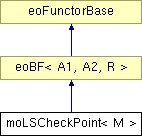
\includegraphics[height=3cm]{classmo_l_s_check_point}
\end{center}
\end{figure}
\subsection*{Public Member Functions}
\begin{CompactItemize}
\item 
void {\bf operator()} (const M \&\_\-\_\-move, const typename M::EOType \&\_\-\_\-sol)
\begin{CompactList}\small\item\em Function which launches the checkpointing. \item\end{CompactList}\item 
void {\bf add} ({\bf eo\-BF}$<$ const M \&, const typename M::EOType \&, void $>$ \&\_\-\_\-f)
\begin{CompactList}\small\item\em Procedure which add a new function to the function vector. \item\end{CompactList}\end{CompactItemize}
\subsection*{Private Attributes}
\begin{CompactItemize}
\item 
std::vector$<$ {\bf eo\-BF}$<$ const M \&, const typename M::EOType \&, void $>$ $\ast$ $>$ {\bf func}\label{classmo_l_s_check_point_ff2a31ee5689a804bd9a572c51a36ca4}

\begin{CompactList}\small\item\em vector of function \item\end{CompactList}\end{CompactItemize}


\subsection{Detailed Description}
\subsubsection*{template$<$class M$>$ class mo\-LSCheck\-Point$<$ M $>$}

Class which allows a checkpointing system. 

Thanks to this class, at each iteration, additionnal function can be used (and not only one). 



Definition at line 21 of file mo\-LSCheck\-Point.h.

\subsection{Member Function Documentation}
\index{moLSCheckPoint@{mo\-LSCheck\-Point}!operator()@{operator()}}
\index{operator()@{operator()}!moLSCheckPoint@{mo\-LSCheck\-Point}}
\subsubsection{\setlength{\rightskip}{0pt plus 5cm}template$<$class M$>$ void {\bf mo\-LSCheck\-Point}$<$ M $>$::operator() (const M \& {\em \_\-\_\-move}, const typename M::EOType \& {\em \_\-\_\-sol})\hspace{0.3cm}{\tt  [inline]}}\label{classmo_l_s_check_point_2f9c1250279e3f49ec77a66c10029f1e}


Function which launches the checkpointing. 

Each saved function is used on the current move and the current solution.

\begin{Desc}
\item[Parameters:]
\begin{description}
\item[{\em \_\-\_\-move}]a move. \item[{\em \_\-\_\-sol}]a solution. \end{description}
\end{Desc}


Definition at line 34 of file mo\-LSCheck\-Point.h.

References mo\-LSCheck\-Point$<$ M $>$::func.\index{moLSCheckPoint@{mo\-LSCheck\-Point}!add@{add}}
\index{add@{add}!moLSCheckPoint@{mo\-LSCheck\-Point}}
\subsubsection{\setlength{\rightskip}{0pt plus 5cm}template$<$class M$>$ void {\bf mo\-LSCheck\-Point}$<$ M $>$::add ({\bf eo\-BF}$<$ const M \&, const typename M::EOType \&, void $>$ \& {\em \_\-\_\-f})\hspace{0.3cm}{\tt  [inline]}}\label{classmo_l_s_check_point_66be5fe2944bcdd752f1e58105e969a6}


Procedure which add a new function to the function vector. 

The new function is added at the end of the vector. \begin{Desc}
\item[Parameters:]
\begin{description}
\item[{\em \_\-\_\-f}]a new function to add. \end{description}
\end{Desc}


Definition at line 49 of file mo\-LSCheck\-Point.h.

References mo\-LSCheck\-Point$<$ M $>$::func.

The documentation for this class was generated from the following file:\begin{CompactItemize}
\item 
mo\-LSCheck\-Point.h\end{CompactItemize}
